\documentclass{beamer}
\usepackage[slovene]{babel}
\usepackage[utf8]{inputenc}
\usepackage[T1]{fontenc}

\usepackage{amsmath}
\usepackage{amsthm}
\usepackage{amsfonts}
\usepackage{url}
\usepackage{graphicx}
\usepackage{enumerate}
\usepackage{listings}
\graphicspath{ {images/} }
 
 
%Information to be included in the title page:
\title{VS postopek za izračun vrednosti polinomov več spremenljivk}
\author{Janez Radešček, Miha Avsec}
\institute{Fakulteta za matematiko in fiziko}
\date{2019}
 
\usetheme{Berlin}
 
 
\begin{document}
 
\frame{\titlepage}

\begin{frame}
\frametitle{Polinom v Bernstein-Bezierjevi obliki (BB)}
Naj bo $T$ trikotnik, potem polinom v baricentričnih koordinatah $(r,s,t)$ lahko zapišemo kot
$$p(r,s,t) = \sum_{i=0}^{d}\sum_{j=0}^{i}b_{d-i,i-j,j}B_{d-i,i-j,j}^{d},$$
kjer je
$$B_{i,j,k}^{d}(r,s,t) = \frac{d!}{i!j!k!}r^is^jt^k$$
Bernsteinov polinom stopnje $d$.

\end{frame}

\begin{frame}[fragile]
\frametitle{De Casteljau}
\begin{block}{De Casteljaujev algoritem}
\begin{lstlisting}[escapeinside={(*}{*)}]
for k=1:d
  for i=0:d-k
      for j=0:i
          (*$b_{d-i-k,i-j,j}^k = r*b_{d-i-k+1,i-j,j}^{k-1}+s*b_{d-i-k,i-j+1,j}^{k-1}$*) 
          	+(*$r*b_{d-i-k,i-j,j+1}^{k-1}  $*)
(*$p(r,s,t) = b_{0,0,0}^{d}$*)
\end{lstlisting}
\end{block}
Algoritem potrebuje $d(d+1)(d+2)/2$ množenj.
\end{frame}



\begin{frame}
\frametitle{Modificirana Bernstein-Bezierjeva oblika polinoma (MBB)}
Polinom v Bernsteinovi obliki lahko zapišemo kot
$$p(r,s,t) = \sum_{i=0}^{d}\sum_{j=0}^{i}c_{d-i,i-j,j}r^{d-i}s^{i-j}t^j,$$
kjer za $c_{d-i,i-j,j}$ vzamemo
$$c_{d-i,i-j,j} = \frac{d!}{(d-i)!(i-j)!j!}b_{d-i,i-j,j}, \quad j=0,\ldots, i; i = 0,\ldots,d.$$
\end{frame}


\begin{frame}
\frametitle{Modificirana Bernstein-Bezierjeva oblika polinoma}
Razdelitev domenskega trikotnika v primeru, ko je $d=2$
\begin{center}
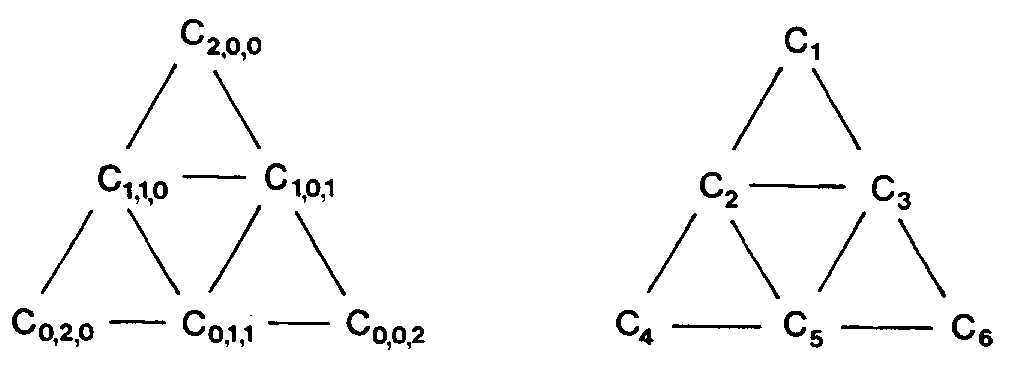
\includegraphics[width=.9\linewidth]{graf.png}
\end{center}

\end{frame}

\begin{frame}
\frametitle{Modificirana Bernstein-Bezierjeva oblika polinoma}
Razvoj po spremenljivki r:
\begin{align}
p(r,s,t) &= \sum_{i=0}^{2}\sum_{j=0}^{i}c_{2-i,i-j,j}r^{2-i}s^{i-j}t^j \nonumber \\ \nonumber
&= r^2\sum_{j=0}^{0}c_{2,-j,j}s^{-j}t^j + r\sum_{j=0}^{1}c_{1,1-j,j}s^{1-j}t^j + \sum_{j=0}^{2}c_{0,2-j,j}s^{2-j}t^j \\ \nonumber
&= r^2(c_1) + r(c_2s+c_3t) + (c_4s^2+c_5st+c_6t^2)\\ \nonumber
&= r^2(c_1+\frac{s}{r}c_2+\frac{t}{r}c_3+\frac{s^2}{r^2}c_4+\frac{st}{r^2}c_5+\frac{t^2}{r^2}c_6) \\ \nonumber
&= r^2(\frac{s}{r}(c_2+\frac{s}{r}c_4+\frac{t}{r}c_5)+\frac{t}{r}(\frac{t}{r}c_6+c_3)+c_1) \nonumber
\end{align}
\end{frame}

\begin{frame}[fragile]
\frametitle{Modificiran Bernstein-Bezierjev algoritem}
\begin{block}{VS algoritem}
\begin{lstlisting}[escapeinside={(*}{*)}]
sr = s/r,	 tr= s/r
A = (*$c_{0,d,0}$*);
for i = 1:d
    B = (*$c_{0,d-i,i}$*)
    for j = i:-1:1
        B = B*tr + (*$c_{i-j+1,d-i,j-1}$*);
    A = A *sr +B;
p(r,s,t) = A(*$r^d$*)
\end{lstlisting}
\end{block}
Algoritem potrebuje $(d^2+5d)/2$ množenj


\end{frame}

\begin{frame}
\frametitle{Izbira spremenljivke}
\begin{center}
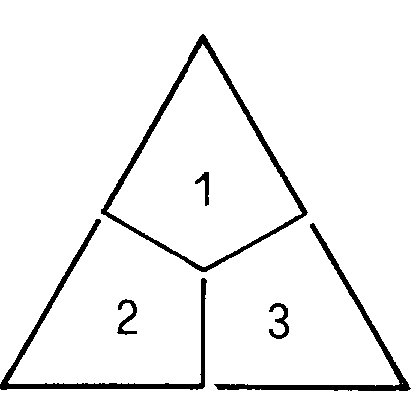
\includegraphics[width=.3\linewidth]{graf1.png}
\end{center}

Posamezne regije so določena na sledeč način
\begin{enumerate}
\item  $r \geq s, r \geq t$
\item $s > r, s \geq t$
\item $t>r, t>s$
\end{enumerate}

\end{frame}

\begin{frame}
\frametitle{Taylor}
Zapis polinoma v Taylorjevi obliki
$$p(u,v) = \sum_{i = 0}^d{\sum_{j=0}^{d-i}{a_{i,j}u^iv^j }}$$
\end{frame}



\begin{frame}[fragile]
\frametitle{Taylorjev algoritem}

\begin{block}{Taylorjev algoritem}
\begin{lstlisting}[escapeinside={(*}{*)}]
p = (*$a_{0,d}$*)
for i = 1:d
    A = (*$a_{i,d-i}$*)
    for j = 1:i
        A = A * u + (*$a_{i-j,d-i}$*)
    end
    p = p * v + A
end
\end{lstlisting}
\end{block}
Algoritem potrebuje $(d^2+3d)/2$ množenj.

\end{frame}

\begin{frame}
\frametitle{Primerjava metod}

\begin{center}
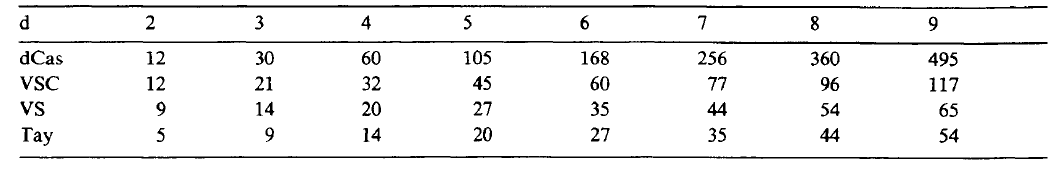
\includegraphics[width=1.0\linewidth]{tabelca.PNG}
\end{center}

\begin{itemize}
\item dCas: De Casteljoujev algoritem
\item VS: algoritem za polinom v MBB olbiki
\item VSC: VS $+$ pretvorba baz
\item Tay: Taylorjev algoritem
\end{itemize}


\end{frame}

\begin{frame}
\frametitle{Polinom v treh spremenljivkah}
Naj bo T tetraeder v $\mathbb{R}^3$ in naj bodo $(r,s,t,u)$ pripadajoče baricentrične koordinate točke $P$. Potem lahko polinom v točki $P$ zapišemo kot
$$p(r,s,t,u) = \sum_{i=0}^{d}\sum_{j=0}^{i}\sum_{k=0}^{j}c_{d-i,i-j,j-k,k}r^{d-i}s^{i-j}t^{j-k}u^{k}.$$
\end{frame}


\begin{frame}
\frametitle{Polinom v treh spremenljivkah}
\begin{center}
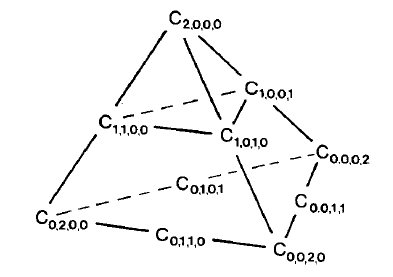
\includegraphics[width=0.7\linewidth]{tetraeder.PNG}
\end{center}
\end{frame}

\begin{frame}[fragile]
\frametitle{Algoritem za polinom v treh spremenljivkah}
\begin{lstlisting}[escapeinside={(*}{*)}]
ru = r/u,	 su= s/u	 tu= t/u
A = (*$c_{d,0,0,0}$*);
for i = 1:d
    B = (*$c_{d-i,i,0,0}$*)
    for j = 1:i
        C =  (*$c_{d-i,i-j,j,0}$*)
            for k = 1:j
                C = C * tu + (*$c_{d-i,i-j,j-k,k}$*)
        B = B * ru + C
    A = A * ru + B;
p(r,s,t,u) = A(*$u^d$*)
\end{lstlisting}
\end{frame}































\end{document}